\documentclass[12pt, a4paper]{article}
\usepackage[left=2cm,right=2cm,top=2cm,bottom=2cm]{geometry}
\usepackage{lastpage}
\usepackage{fancyhdr}
\usepackage{parskip}
\usepackage{datetime}
\usepackage{datenumber}
\usepackage{advdate}
\usepackage{enumitem}
\usepackage{url}
\usepackage{hyperref}
\usepackage{footnote}
\usepackage{color}  
\usepackage{titlesec}
\usepackage[super]{nth}
\usepackage{pdfpages}



\titleformat{\section}{\large\bfseries}{\thesection}{1em}{}
\titleformat{\subsection}{\normalsize\bfseries}{\thesection}{1em}{}

\titlespacing\section{0pt}{8pt plus 4pt minus 2pt}{0pt plus 2pt minus 2pt}


\titlespacing\subsection{0pt}{8pt plus 4pt minus 2pt}{0pt plus 2pt minus 2pt}

\renewcommand\labelitemi{--}

\setlength{\headheight}{15pt}
\renewcommand{\headrulewidth}{0pt}

% Specify date format like "15th Oct"
\newdateformat{datefmt}{\nth{\THEDAY} \shortmonthname[\THEMONTH]}

% Force advdate commands to change the global "today" instance, not the local one
\makeatletter
\renewcommand\AdvanceDate[1][\@ne]{\global\advance\day#1 \FixDate}
\renewcommand\FixDate{%
  \FixMonth \is@LeapYear
  \l@@p \global\ifnum\day<1 \Pr@vD@y \repeat
  \l@@p \M@s\m@sic \global\ifnum\day>\M@s \N@xtD@y \repeat
}
\renewcommand\FixMonth{%
  \L@@p \global\ifnum\month<1 \global\advance\year\m@ne \global\advance\month12 \is@LeapYear \repeat
  \L@@p \global\ifnum\month>12 \global\advance\year\@ne \global\advance\month-12 \is@LeapYear \repeat}
\def\Pr@vD@y{%
  \global\ifnum\day<-366
    \global\ifnum\month>2
      \global\advance\day\r@k \global\advance\year\m@ne \is@LeapYear
    \else
      \global\advance\year\m@ne \is@LeapYear \advance\day\r@k
    \fi
  \else
    \global\advance\month\m@ne \FixMonth
    \global\advance\day\m@sic
  \fi}
\def\N@xtD@y{%
  \global\ifnum\day>366
    \global\ifnum\month>2
      \global\advance\year\@ne \is@LeapYear \global\advance\day-\r@k
    \else
      \global\advance\day-\r@k \global\advance\year\@ne \is@LeapYear
    \fi
  \else
    \global\advance\day-\M@s \global\advance\month\@ne \FixMonth
  \fi}
\makeatother

% Output eg. boldface "15th Oct - 29th Oct" when called.
\newcommand{\daterange}[1]{%
    \textbf{\datefmt \today}
    \textbf{--}
    \AdvanceDate[#1]\relax
    \AdvanceDate[-1]\relax
    \textbf{\datefmt \today}
    \AdvanceDate[1]\relax
}

\pagestyle{fancy} 

\cfoot{\thepage\ of \pageref{LastPage}}
\lhead{}
\rhead{}

\setlength{\parskip}{0.5em}
\setitemize{itemsep=-0.3em}

\begin{document}

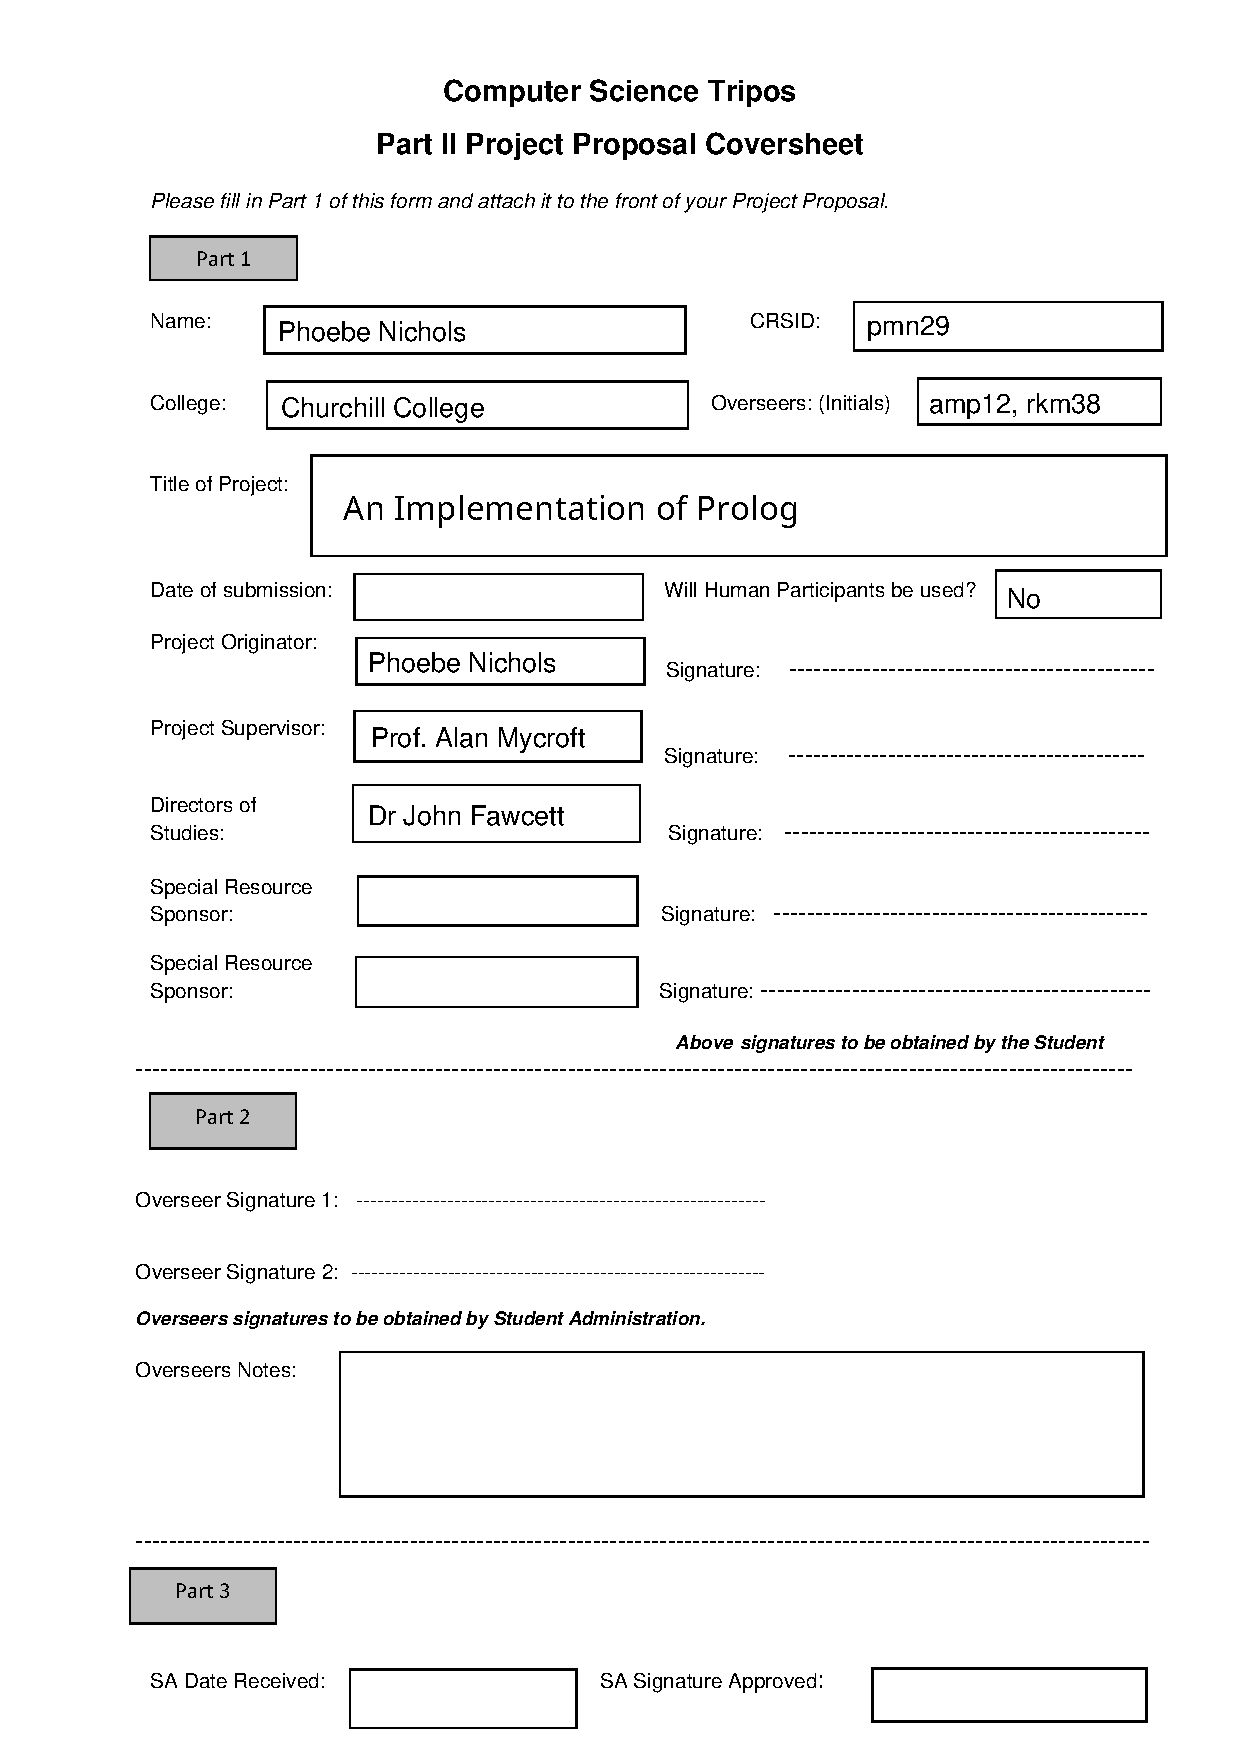
\includepdf[pages=-]{ProposalForm}

\clearpage
\setcounter{page}{1}



\centerline{\large Computer Science Tripos: Part II Project Proposal}
\vspace{2em}
\centerline{\Large\bf A Prolog Compiler and Abstract Machine}
\vspace{2em}
\centerline{Phoebe Nichols, pmn29}
\centerline{Churchill College}
\centerline{October 2018}

\vspace{2em}

\begin{center}
\begin{tabular}{ l l l l }
{\bf Project Originator:} & Phoebe Nichols & {\bf Project Supervisor:} & Prof. Alan Mycroft \\[3mm]
{\bf Director of Studies:} & Dr John Fawcett & {\bf Overseers:} & Prof. Andrew Pitts \\[3mm]
&&&  Dr Rafal Mantiuk  \\[3mm]
\end{tabular}
\end{center}



\section*{Introduction and Description of the Work}

Prolog is a declarative programming language. This means that a Prolog programmer declares rules that describe the result of a program, but does not specify how the program should achieve this result. This is in contrast to imperative programming languages such as Java, where the programmer specifies how a program's state should be changed in order to achieve the result of the program. The use of a declarative language presents the interesting problem of how to evaluate a query without being told how the answer to the query should be computed. In the case of Prolog, this problem is solved by performing a graph search over the Horn clauses given in a Prolog program. This graph search attempts to find an assignment of values to variables that satisfies the query, or rejects the query if no such assignment exists. Typically, a left-to-right depth-first search is performed.

The aim of this project is to implement a compiler and abstract machine for Prolog. The target for the Prolog compiler will be specialised byte-code. Designing this byte-code will form part of the project. The abstract machine implemented will interpret this byte-code to run the original Prolog program. An existing specification of an abstract machine to execute Prolog, the Warren Abstract Machine (WAM), will be used as inspiration---but I will not implement the full WAM.

The project will be restricted to a basic subset of Prolog so that it remains feasible. Some extensions that I am considering (for example type checking) will require an extension to Prolog syntax in order to provide information about program properties. The syntax I use may therefore not be a true subset of standard Prolog.


\section*{Starting Point}

\subsection*{Prolog as a programming language}

I will need a good understanding of how to program in Prolog in order to implement the Prolog compiler. I will also need to write test programs for the subset of Prolog that I have chosen to compile. These tests will help me to evaluate the correctness and performance of my compiler and abstract machine implementation.

I am studying the 50\% course, which does not cover Prolog until Lent term this year. I have, therefore, studied the Prolog course over the summer.

\subsection*{Prolog compilation and execution}

I have no prior experience with implementing Prolog interpreters or compilers. The IB 75\%/II 50\% Prolog course that I studied over the summer introduced me to the basics of Prolog execution. I have also read around this area over the summer: some of the papers I read are cited in this document.

\subsection*{OCaml}

I am intending to implement all of my project in OCaml initially, although I may add some SWI-Prolog for extension features. I have chosen OCaml because I have experience implementing lexers and parsers in ML from the compilers course, and found ML convenient for this sort of thing. OCaml will have same advantages as ML, but is more widely used and therefore has more tools and libraries available. 

I have very little prior experience with OCaml (only from the IB compilers course), so I will need to dedicate time to studying it. This time is provisioned in my project plan.

\section*{Structure of the Project}

The project is made up of four main components:
\begin{enumerate}
\item Lexer
\item Parser
\item Translator
\item Abstract machine
\end{enumerate}

I will implement the components in this order. This is because each component can be used to generate test cases for the next component. As an extension, I may add a semantic analysis phase acting on the parse tree. This would verify program properties and try to provide information so that the translator can generate more efficient code.

\subsection*{Testing}

Unit tests will be written for each individual component. Components written in OCaml will likely have unit tests written with the testing framework OUnit \cite{OUnit}. Any components written in SWI-Prolog will be tested using native support for unit tests as described in the SWI-Prolog documentation \cite{PUnit}. I will write unit tests for each component along with the implementation of the component itself.
   
\subsection*{Evaluation}
   
I will be able to quantitatively evaluate the project in terms of:
\begin{itemize}
\item The run-time performance of my abstract machine compared to standard Prolog implementations such as SWI-Prolog.
\item The run-time performance of my abstract machine compared to my interpreter.
\item The change in code size, number of choice points, or performance, for any optimisations that I implement.
\end{itemize}
Here, `performance' means a comparison of space and time usage for sample programs. The Spacetime functionality of the OCaml compiler can be used for profiling the memory behaviour of an OCaml program \cite{SpaceT}, and SWI-Prolog includes predicates for execution profiling \cite{PExec}.

\section*{Success Criterion}

My success criterion is to implement the following components for a basic subset of Prolog:

\begin{itemize}
\item Lexer
\item Parser 
\item Translator from parse tree to byte-code 
\item Abstract machine to execute this byte-code
\end{itemize}

These components should enable me to correctly execute example programs written in the grammar that I use. The components will not implement the full ISO Prolog standard, and the grammar used may include features such as type annotations not found in standard Prolog. The lexer and parser might be implemented manually, or using ocamllex and ocamlyacc.

\section*{Possible extensions}

The main extensions for this project involve adding optimisations to the compiler. Some potential optimisations are:
\begin{itemize}
\item \textbf{Last call optimisation} \\
Tail recursion can be converted to iteration to save adding a new stack frame for each tail recursive call. 

\item \textbf{Determinacy analysis} \\
A clause is said to be determinate if it can only return one possible solution \cite{costsBenefitsAbstract}. This information can be used to avoid backtracking through determinate clauses.

\item \textbf{Mode analysis} \\
The argument to a predicate can be assigned a mode to say that the argument is always used as input, or as output \cite{autoMode}. Mode information can be used to invoke special purpose unification routines that test for fewer cases and therefore can be faster.


\item \textbf{Type checking} \\
It is possible to define a polymorphic type system for Prolog \cite{mycroftTypes}. Type information can be used to select faster, special-purpose unification routines. A type checker also has the significant advantage of potentially spotting program bugs and saving developer time.

\end{itemize}
There are many more possible optimisations I could apply, and I might also select one of these for an extension. As I implement the initial system I will learn more about the optimisations I could make, and may also find my implementation to be more suited to certain optimisations.

\section*{Timetable and Milestones}

\ThisYear{2018}\ThisMonth{10}\ThisDay{22}

\daterange{14} \hfill{\emph{\textbf{19\textsuperscript{th} Oct}: Proposal submitted}}

Project set-up:
\begin{itemize}
\item Investigate and set up an IDE for OCaml.
\item Set up a backup system for the project.
\item Choose a software engineering methodology to follow.
\item Learn to use the testing frameworks needed for the project. 
\end{itemize}
Write small programs in SWI-Prolog, to re-enforce understanding of Prolog and for potential use as benchmarks. Study OCaml using the Real World OCaml textbook \cite{ocamlBook}, and write small programs in OCaml to gain familiarity with the language.

Milestones:
\begin{itemize}
\item Document produced to describe the development environment, backup system, software engineering methodology, and testing frameworks used.
\item Example programs written in OCaml.
\item Example programs written in Prolog.
\end{itemize}

\daterange{14} 

Implement a lexer and parser for the chosen subset of Prolog. I am intending to use ocamllex and ocamlyak (described in \cite{ocamlyak}) for this.

Milestones:
\begin{itemize}
\item Code for lexer written and tested.
\item Code for parser written and tested.
\item Document produced to describe the implementation of these components.
\end{itemize}

\daterange{14} 
\hfill{\emph{\textbf{28\textsuperscript{th} Nov}: Last day of Michaelmas term}}

Implement an interpreter to evaluate the parse tree output by the parser. This interpreter will guide the design of the abstract machine, and may be useful as a performance benchmark.

Milestones:
\begin{itemize}
\item Code for interpreter written and tested.
\item Document produced to describe the implementation of the interpreter.
\end{itemize}

\daterange{14} 

Design the byte-code to represent Prolog programs, and write an abstract machine to execute this byte-code. Write the translator to convert the parse tree to byte-code.

Milestones:
\begin{itemize}
\item Code for abstract machine written and tested.
\item Code for translator written and tested.
\item Document produced to describe the byte-code format chosen.
\item Document produced to describe how the abstract machine works.
\end{itemize}

\daterange{7} [\emph{Slack}]

 Read about possible extensions to the project. This could be research on type, mode, or determinacy analysis for Prolog. Of these options I expect type checking to be the most complex, and determinacy analysis the least complex. I will choose where to invest my time depending on how far ahead or behind the project is.

Milestones:
\begin{itemize}[nosep]
\item Produce document to summarise research into optimisations.
\end{itemize}

\daterange{7} [\emph{Christmas break}]

\daterange{7} [\emph{Slack}]

Continue research into extensions.

Milestones:
\begin{itemize}
\item Add more content to the previous summary document.
\end{itemize}

\daterange{14} [\emph{Slack}] \hfill{\emph{\textbf{17\textsuperscript{th} Jan}: First day of Lent term}}

Implement extension features for the compiler.

Milestones:
\begin{itemize}
\item Code for extension features written and tested.
\item Document produced to describe the theory and implementation of the extension features.
\end{itemize}

\daterange{7} 

Prepare for progress report and presentation.

Milestones:
\begin{itemize}
\item Progress report and presentation written.
\end{itemize}

\daterange{14} \hfill{\emph{\textbf{1\textsuperscript{st} Feb}: Progress report deadline}}

Write a draft of the structure of the dissertation, giving the main points to be covered. Write a full version of the evaluation section of the dissertation.

Milestones:
\begin{itemize}
\item Draft structure of dissertation written, and sent to DoS and supervisor.
\item Evaluation section written, and sent to DoS and supervisor.
\end{itemize}


\daterange{14}

Respond to any feedback on the draft structure or evaluation section.

Write the introduction, preparation, implementation, and conclusion sections of the dissertation. I will be able to use material from the documents I intend to produce throughout the project, so I will not have to write these sections from scratch.

Milestones:
\begin{itemize}
\item Dissertation completed, and sent to DoS and supervisor.
\end{itemize}

\daterange{14} [\emph{Slack}]

 I will use this time to finish the dissertation if the first draft is not already finished. If a draft is finished then I will likely be waiting for feedback, and will dedicate this time to revision.

Milestones:
\begin{itemize}
\item If the previous milestone was missed then it should now be met.
\end{itemize}

\daterange{14} \hfill{\emph{\textbf{13\textsuperscript{th} Mar}: Last day of Lent term}}

Respond to any feedback on the dissertation. 

Milestones:
\begin{itemize}
\item Dissertation updated following any feedback received.
\end{itemize}

\daterange{14} [\emph{Slack}]

Continue improving the dissertation and responding to feedback.

Milestones:
\begin{itemize}
\item Dissertation updated.
\end{itemize}

\daterange{14} [\emph{Slack}]

Continue improving the dissertation and responding to feedback.

Milestones:
\begin{itemize}
\item Dissertation updated.
\end{itemize}

\daterange{14}  \hfill{{\emph{\textbf{25\textsuperscript{th} Apr}: First day of Easter term}}}

Make any final changes and submit the dissertation.

Milestones:
\begin{itemize}
\item Dissertation submitted.
\end{itemize}


\rightline{\emph{\textbf{17\textsuperscript{th} May}: Dissertation deadline}}


\section*{Resources Required}

I am intending to use my own laptop for the project (Dell XPS 15, 16GB RAM, i7-7700HQ, running Ubuntu). I accept full responsibility for this machine and I have made contingency plans to protect myself against hardware and/or software failure.

The basic resources that are essential to my project are the OCaml compiler \texttt{ocamlopt} and the SWI-Prolog interpreter \texttt{swipl}. These are both installed on the MCS system. I will be able to complete the project using the MCS machines if my laptop fails.

I will use git for revision control. My git repository will be hosted in GitHub, and this will serve as a cloud backup of my code. I will store my local copy of the git repository inside a Dropbox folder so that my work is also all automatically synced to Dropbox. I will perform weekly backups to a USB stick in case these other backup techniques fail.
       
\bibliographystyle{unsrt}

\bibliography{references}

   

\end{document}
